%\documentclass[mathserif]{beamer}
\documentclass[handout]{beamer}
%\usetheme{Goettingen}
\usetheme{Warsaw}
%\usetheme{Singapore}
%\usetheme{Frankfurt}
%\usetheme{Copenhagen}
%\usetheme{Szeged}
%\usetheme{Montpellier}
%\usetheme{CambridgeUS}
%\usecolortheme{}
%\setbeamercovered{transparent}
\usepackage[english, activeacute]{babel}
\usepackage[utf8]{inputenc}
\usepackage{amsmath, amssymb}
\usepackage{dsfont}
\usepackage{graphics}
\usepackage{cases}
\usepackage{graphicx}
\usepackage{pgf}
\usepackage{epsfig}
\usepackage{amssymb}
\usepackage{multirow}	
\usepackage{amstext}
\usepackage[ruled,vlined,lined]{algorithm2e}
\usepackage{amsmath}
\usepackage{epic}
\usepackage{epsfig}
\usepackage{fontenc}
\usepackage{framed,color}
\usepackage{palatino, url, multicol}
\usepackage{listings}
%\algsetup{indent=2em}


\vspace{-0.5cm}
\title{Introduction to Causal Inference}
\vspace{-0.5cm}
\author[Felipe Bravo Márquez]{\footnotesize
%\author{\footnotesize  
 \textcolor[rgb]{0.00,0.00,1.00}{Felipe José Bravo Márquez}} 
\date{ \today }




\begin{document}
\begin{frame}
\titlepage


\end{frame}


%%%%%%%%%%%%%%%%%%%%%%%%%%%


\begin{frame}{Motivation}
\scriptsize{
\begin{itemize}
\item Our starting point is the difference between an observation and an intervention (or action). 
\item We can answer many questions from passive observation alone.
\item For example: do 16 year-old drivers have a higher incidence rate of traffic accidents than 18 year-old drivers? 
\item The answer corresponds to a difference of conditional probabilities.

\item Let random variables $I,A$ correspond to traffic incident rate and driver's age correspondingly:
\begin{displaymath}
 P(I|A=16)-P(I|A=18)>0?
\end{displaymath}


\item Both conditional probabilities can be estimated from a large enough sample drawn from the distribution.

\item The answer to the question we asked is solidly in the realm of observational statistics.

\item However, important questions often are not observational in nature.

\end{itemize}

\footnotemark{These slides are mainly based on Chapter 9 of \cite{hardt2021patterns}.}

} 

\end{frame}

\begin{frame}{Motivation}
\scriptsize{
\begin{itemize}
\item Causal question:  Would traffic fatalities decrease if we raised the legal driving age by two years? 
\item Here we are not asking for the frequency of an event in our manifested world.
\item This question asks for the effect of a hypothetical \textbf{intervention}.
\item As a result, the answer is not so simple. 
\item Even if older drivers have a lower incidence rate of traffic accidents, this might simply be a consequence of additional driving experience. 
\item There is no obvious reason why an 18 year old with two months on the road would be any less likely to be involved in an accident than a 16 year-old with the same experience.


\end{itemize}

} 

\end{frame}



\begin{frame}{Motivation}
\scriptsize{
\begin{itemize}
\item We can try to address this problem by holding the number of months of driving experience fixed, while comparing individuals of different ages.
\item But we quickly run into subtleties.
\item What if 18 year-olds with two months of driving experience predominantly live in regions where traffic conditions differ significantly from those in areas where people feel a greater need to drive at a younger age?

\item  Causal reasoning is a conceptual and technical framework for addressing questions about the effect of hypothetical actions or interventions. 
\item Once we understand what the effect of an intervention is, we can turn the question around and ask what action plausibly caused an event. 
\item This gives us a formal language to talk about cause and effect.


\end{itemize}

} 

\end{frame}


\begin{frame}{The limitations of observation}
\scriptsize{
\begin{itemize}
\item Before we develop any new formalism, it is important to understand why we need it in the first place.
\item To see why we turn to the  example of graduate admissions at the University of California, Berkeley  \cite{bickel1975sex}.

\item The aggregate admission decisions of the six largest departments at the University was compared between male and female applicants. 
\item The aggregated acceptance rate for these six departments is 44\% for men and 30\% for women.

\item The difference is statistcally significant. 
\item  This led to an investigation into whether the University was acting in a gender-discriminatory manner.

\item Recognizing that departments have autonomy over who to admit, we can look at the gender bias of each department.


\end{itemize}

} 

\end{frame}

\begin{frame}{The limitations of observation}
\scriptsize{
\begin{figure}[h!]
	\centering
	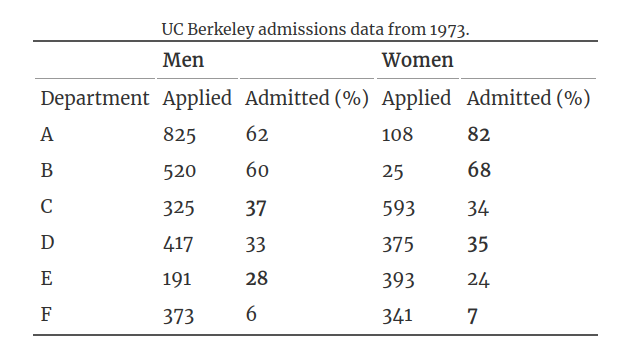
\includegraphics[scale=0.4]{pics/berkley.png}
\end{figure}

\begin{itemize}

\item Four of the six largest departments show a higher acceptance ratio among women.
\item The two other departments with higher acceptance rate for men cannot account for the large difference in acceptance rates that we observed in aggregate. 
\item It appears that the higher acceptance rate for men that we observed in aggregate seems to have reversed at the department level.


\end{itemize}

} 

\end{frame}


\begin{frame}{The limitations of observation}
\scriptsize{

\begin{itemize}

\item Such reversals are sometimes called Simpson's paradox. 
\item Even though mathematically they are no surprise.
\item It's a fact of conditional probability that there can be events $Y$ (acceptance), $A$ (gender) and a random variable $Z$ (department choice) such that:
\begin{enumerate}
\scriptsize{
 \item $\mathbb{P}(Y|A)  < \mathbb{P}(Y|\neg A)$
 \item $\mathbb{P}(Y|A, Z =z)  > \mathbb{P}(Y|\neg A,Z=z)$ for all values $z$ that the random variable $Z$ assumes.}
\end{enumerate}
\item Simpson's paradox nonetheless causes discomfort to some.

\item Intuition suggests that a trend which holds for all subpopulations should also hold at the population level.


\end{itemize}

} 

\end{frame}



%%%%%%%%%%%%%%%%%%%%%%%%%%%
\begin{frame}[allowframebreaks]\scriptsize
\frametitle{References}
\bibliography{bio}
\bibliographystyle{apalike}
%\bibliographystyle{flexbib}
\end{frame}  









%%%%%%%%%%%%%%%%%%%%%%%%%%%

\end{document}
